Als we terminal opstarten dan komen we in PowerShell terecht.

\begin{minipage}[t]{\linewidth}
\raggedright
\adjustbox{valign=t}{%
	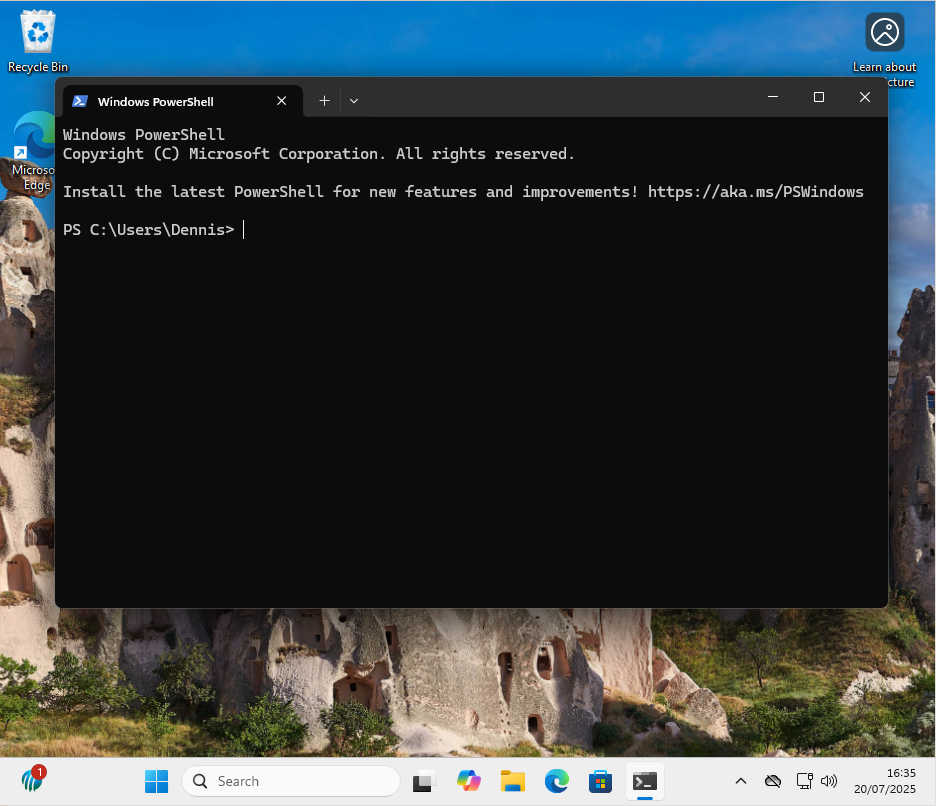
\includegraphics[width=0.99\linewidth]{Terminal_PS.png}%
}
\end{minipage}
Aan de linkerkant van het Terminal window zien we een knipperende cursor. Voor deze cursor vinden we een regel die begint met PS, om aan te geven dat we in PowerShell werken. Als er niets staat dan maken we gebruik van \texttt{cmd}. Na de PS zien we C:, dit is onze C-drive. Je kunt je nu afvragen waar de A en de B-drive gebleven zijn. Dat is geen vreemde vraag. Het Windows besturingssysteem bestaat al lang en in een grijs verleden waren er floppy disks en deze disks moest je plaatsen in een, meestal ingebouwde, floppy drive. De eerste twee drive letters waren gereserveerd voor deze floppy drives. De eerste harddisk in een systeem kreeg daardoor de letter C en dat is altijd zo gebleven. De C-drive is de disk waarvan het systeem is opgestart. Hierop staat Windows op en alles wat daarbij hoort.

Het laatste stuk bestaat uit \texttt{\textbackslash Users\textbackslash Username}. Dit is het pad waarin je staat. Username is bij jou vervangen door de naam waarmee je ingelogd bent. Als je ingelogd bent als Administrator dan is het pad: \texttt{\textbackslash WINDOWS\textbackslash system32}. In de laatste geval adviseren zou je eigenlijk moeten uitloggen en inloggen als gewone gebruiker. Als Administrator heb je te veel rechten en kan je te veel stuk maken.

